\documentclass[autodetect-engine,dvi=dvipdfmx,ja=standard,twocolumn,jbase=13.35Q]{bxjsarticle} 
% 日本語, LaTeXエンジン自動判定, 欧文9.5pt=和文13.35Q
%\documentclass[twocolumn,dvipdfmx]{jsarticle} % (古いので廃止) pLaTeX+dvipdfmxユーザ用
%\documentclass[a4paper,twocolumn]{article} % for English only manuscript

%%%%%%%%%%%%%%%%%%%%%%%%%%%%%%%%%%%%%%%%%%%%%%%%%%%%%%%%%
%% <local definitions here>
\usepackage{comment}
\usepackage[hang,small,bf]{caption}
\usepackage[subrefformat=parens]{subcaption}
\captionsetup{compatibility=false}

\usepackage{latexsym}
\usepackage{graphicx}
\usepackage{amssymb,amsmath}
\usepackage{url}
%% 本文と数式のフォントをTimes(注:New Romanではない)互換フォントにする。
%% AMS(数学)関係のパッケージのusepackageよりも後に置くこと。(前に置くと、
%% AMS関係のパッケージをusepackageしたところでエラーになるので注意)
\usepackage{newtxtext}
\usepackage[varg]{newtxmath}
%% PDFのメタデータにTitleとAuthorを入れる。
\usepackage[pdfusetitle]{hyperref}
%% 行間を詰める。
\renewcommand{\baselinestretch}{0.9}
%% itemize, enumerate, descriptionに追加される行間をなくす。
% \usepackage{enumitem}
% \setlist{topsep=0pt,parsep=0pt,partopsep=0pt,itemsep=0pt}


%% </local definitions here>
%%%%%%%%%%%%%%%%%%%%%%%%%%%%%%%%%%%%%%%%%%%%%%%%%%%%%%%%%

%--------卒業研究予稿集用スタイルファイルのパラメタ ここから--------
\usepackage{jcourse-proceeding}
\jcpnumber{C--1--6} % 発表番号
\title{頭部伝達関数の機械学習に基づく\\
前後方向の音像識別に関する検討}% 卒業研究の題目
%\jcpsubtitle{(タイトルの下に付加情報を付けられます。太字。中央配置。サブタイトルなど。例→) 良かったら卒業研究以外にも使ってください}
\author{瀬音 光一} % 発表者氏名
\jcplaboratory{(永田研究室)} % 研究室名
%\jcpunderauthor{(著者の下に付加情報を付けられます。普通字。左寄せ。タイトル領域で特に言及したい文献情報など。例→) T. Iwate, H. Morioka, and G. Ueda, ``This is a sample title of an article in some journal or conference,'' \emph{International Journal of Something}, Vol.3, No.11, pp.110--118, Jan. 2020. }


%\jcpabstract{}
%--------卒業研究予稿集用スタイルファイルのパラメタ ここまで--------

\begin{document}
\maketitle

%%%%%%%%%%%%%%%%%%%%%%%%%%%%%%%%%%%%%%%%%%%%%%%%%%%%%%%%%%%%%%%%
\section{はじめに}
%%%%%%%%%%%%%%%%%%%%%%%%%%%%%%%%%%%%%%%%%%%%%%%%%%%%%%%%%%%%%%%%
前後方向の音像の識別には、頭の形、特に耳介の形
と前後の非対称性が大きく影響していることが知られている。
この非対称により、同一の信号音でも前方から来た場合と後方から来た場合とでは、
各々の周波数特性が異なる。
この周波数特性上の方向定位に関する手掛かりをスペクトルキューと呼び、
前後方向のスペクトルキューについては、頭部伝達関数(HRTF:Head-Related Transfer Fuction)
の4kHz付近に存在するピーク(P1)、及び4kHz以上に存在する最初のノッチ(N1)とその次の
ノッチ(N2)が知られているが\cite{K}、
HRTFは音源の信号が既知でないと推定できないはずであり、
またスペクトル上のノッチは背景雑音によって容易に消失してしまうため、
ヒトがノイズの存在する環境の中でその差異をどのように識別し、学習しているかは明らかではない。
%HRTFではなく両耳間レベル差(ILD:Interaural Level Difference)
そこで、本研究では
%実世界においては従来のHRTFではなく、両耳間の相関によってヒトは前後の識別を学習していると考え、
特に音像制御の難度が高いとされている前後の定位\cite{K2}について
機械学習を用いてその学習が可能であるかを検討する。

%%%%%%%%%%%%%%%%%%%%%%%%%%%%%%%%%%%%%%%%%%%%%%%%%%%%%%%%%%%%%%%%
\section{断片的な信号音による到来方向識別}
%%%%%%%%%%%%%%%%%%%%%%%%%%%%%%%%%%%%%%%%%%%%%%%%%%%%%%%%%%%%%%%%

音響伝達関数推定に使われる掃引正弦波や白色雑音といった人工的な信号を方向識別の学習信号として用いれば、
%精度の高いHRTFが推定可能であり、これを用いれば
前後の識別は比較的容易であると考えられるが、ヒトは測定用信号ではなく、
時間的にも周波数の上でも断片的で片寄った信号から到来方向に関する学習を行っているものと考えられる。
また先述したように、
HRTFは音源の信号が既知でないと推定できないはずであり、
背景雑音が伝達関数上のノッチを隠し、さらに学習の精度を低下させるものと考えられる。

そこで、本研究では伝達関数測定用の人工的な信号ではなく、
実世界で到来するような断片的な信号から不完全な前後のHRTFと両耳間レベル差(ILD:Interaural Level Difference)の集合を求め、
これらを入力とした機械学習による前後の識別について検討する。
%前後の識別がそれらの機械学習によって可能か各々検討する。\\
     
\begin{comment}
     掃引正弦波や白色雑音といった人工的な信号を用いれば、精度の高い頭部伝達関数が推定可能であり、
     これを用いれば前後の識別は比較的容易であると考えられる。
     実際に、掃引正弦波と白色雑音、220の信号の頭部伝達関数を求めたところ、
     掃引正弦波と白色雑音には先述した特徴を確認することができ、前後の識別も可能であった。
     しかし、220の信号に関しては、その特徴が確認できず前後の識別も困難であった。
     これは、220の信号が時間的にも周波数的の上でも断片的で片寄った信号であるためだと考えられる。

     そこで、本研究では伝達関数測定用の人工的な信号ではない
     実世界で到来するような断片的な信号で、
     なお且つスピーカーの伝達関数を考慮しなくてよい両耳間レベル差の不完全な前後の集合を求め、
     前後の識別がそれらの機械学習によって、可能か検討する。\\
\end{comment}

\subsection{前後の頭部伝達関数の測定}
HRTF推定に使用した音源は、音声、効果音、ボーカル入り音楽の3種類で時間長は各々3秒弱である。
音源の内訳は、音声72、効果音60、音楽88、合計220であり、
録音はダミーヘッドの両耳にマイクロホンを装着し、図\ref{fig:0}に示す環境で行った。
また、録音信号には別途ダミーヘッドで録音した左右の背景雑音をSN比10dBとなるように加えた。
%HRTFは$El,r$と$F$とのクロススペクトル法により算出した。
%ここで、添字の$l$、$r$は各々左右の耳を表し、$E$と$F$は各々
背景雑音を加えた録音信号および、音源信号に対し
1024点のDFTスペクトルから
%により得られた512点の複素数から
クロススペクトル法によりHRTFを算出した。

%\\$HRTFl,r(w) = El,r(w)/ F(w) (1)$\\
\begin{comment}
\begin{equation}
     HRTFl,r(w) = El,r(w)/ F(w)
     %HRTF(w) = \frac{\overline{ Y(w)*X(w)^{*} }}{ \overline{ X(w)*X(w)^{*} }}
\end{equation}
\end{comment}

上記の環境で、白色雑音と220の信号からHRTFを求めた。
白色雑音のHRTFを図\ref{fig:whitenoiseHRTF}に、
220の信号ごとに得られたHRTFのうち例として3つを図\ref{fig:HRTF}に示す。
図\ref{fig:whitenoiseHRTF}と図\ref{fig:HRTF}を比べると、
白色雑音では、6kHz付近のノッチで前後の判断が可能であり先行研究\cite{K}と一致する結果が得られた。
一方、雑音重畳両耳録音信号からは前後の特徴を見出すことが困難であった。

\begin{comment}
一方、図\ref{fig:A}から分かるように、実音源による伝達関数は雑音ののような振幅のばらつきがあり、
そのままでは差異の確認が難しいため、
目視でも差異を確認できるようにスムージングを行った。その結果を図\ref{fig:B}に示す。
その結果、図\ref{fig:B}の四角部分に違いを確認できる。
スムージングには、Savizky-Golay法を使用した。
\end{comment}

\begin{comment}
特徴が見られる8kHz~15kHz区間だけ出力したものが図\ref{fig:C}になる。
この区間で機械学習による識別を行うことにした。

\begin{table}[htbp]
     \centering
     \begin{tabular}{l|c}
       分類 & 音源数  \\ \hline\hline
       音声 & 72  \\
       効果音 & 60  \\
       音楽(ボーカル有り) & 88  \\ \hline
       合計 & 220 \\
     \end{tabular}
     \caption{音源の分類}
     \label{tb:fugafuga1}
\end{table}
\end{comment}

\begin{figure}[htbp]
     \begin{center}
     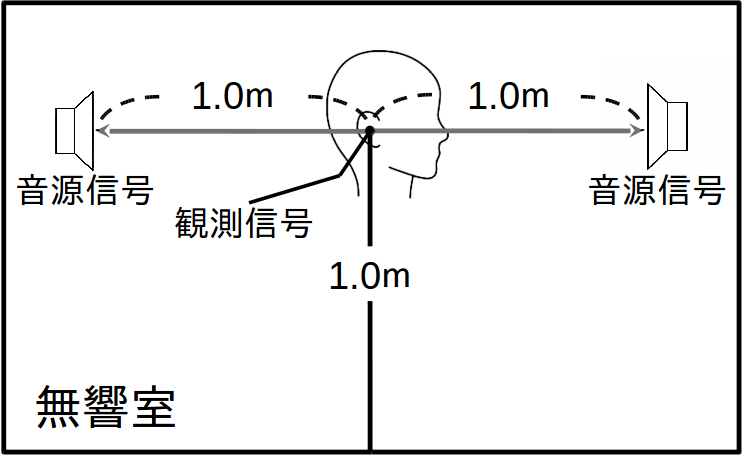
\includegraphics[clip, width=2.0in, height = 0.9in]{picture/environment.png}
     \end{center}
     \caption{録音環境}\label{fig:0}
\end{figure}

\begin{comment}
\begin{figure}[htbp]
     \begin{center}
     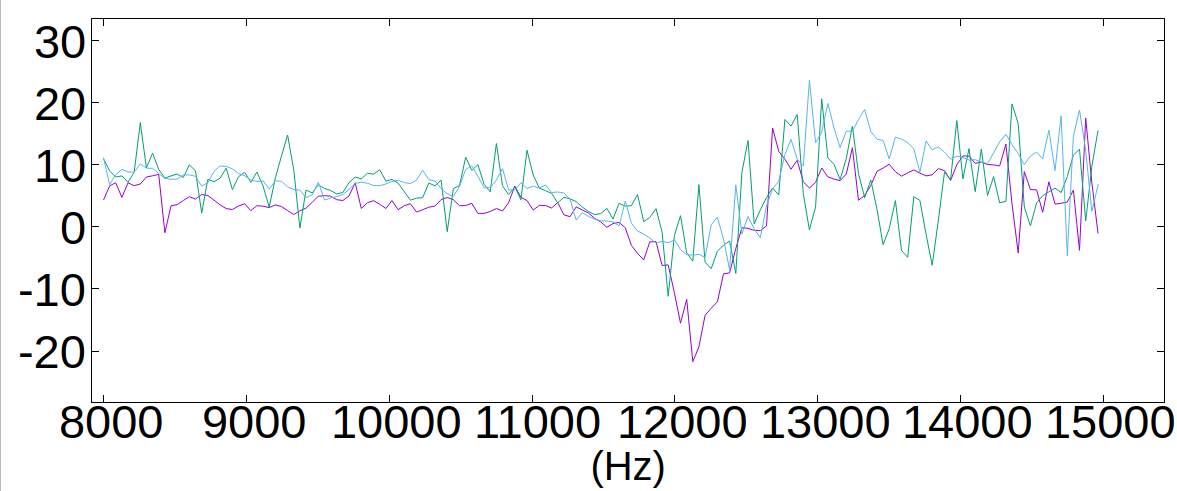
\includegraphics[clip, width=3.2in, height = 1.5in]{picture/mae_limit_NoSmoothing.png}
     \subcaption{音源が前方の場合}
     
     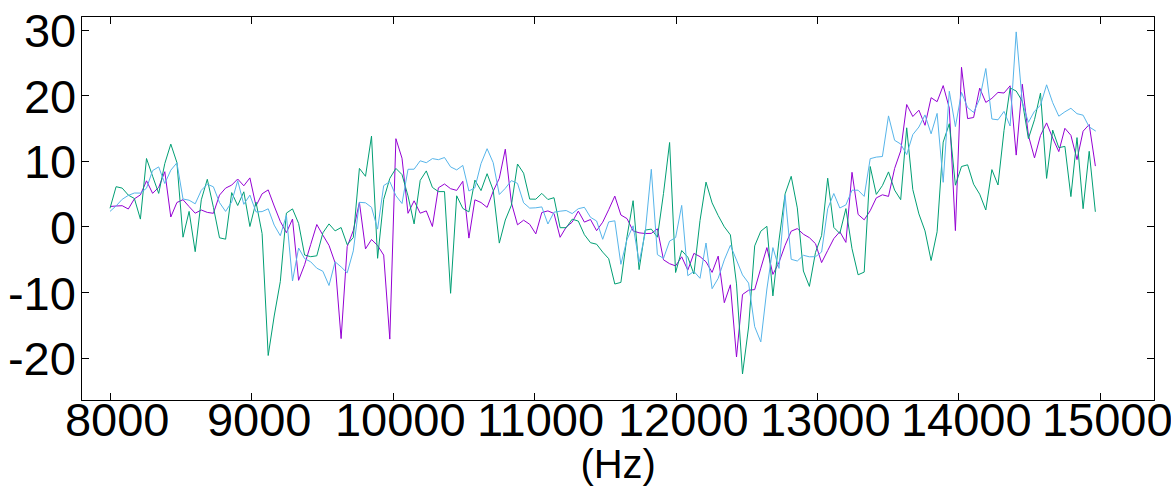
\includegraphics[clip, width=3.2in, height = 1.5in]{picture/usiro_limit_NoSmoothing.png}
     \subcaption{音源が後方の場合}
     \end{center}
     \caption{8kHz〜15kHz区間の両耳間レベル差}\label{fig:C}
\end{figure}

\end{comment}



\subsection{前後の両耳間レベル差の測定}
ILDもHRTFと同様に、左耳の録音信号と右耳の録音信号から1024点のDFTによる
クロススペクトル法を用いて算出した。
%添字の$l$、$r$は各々左右の耳を表し、
%$E$は背景雑音を加えた録音信号を1024サンプルでDFTした512サンプルの複素数である。
白色雑音の両耳間レベル差を図\ref{fig:whitenoiseILD}に、
220の信号ごとに得られた両耳間レベル差のうち例として3つを図\ref{fig:AILD}に示す。
図\ref{fig:whitenoiseILD}と図\ref{fig:AILD}を比べると
どちらも10kHz付近で前後の差異が確認できる。


\begin{comment}
\begin{equation}
     ILDl,r(w) = El(w)/ Er(w)
          
     %HRTF(w) = \frac{\overline{ Y(w)*X(w)^{*} }}{ \overline{ X(w)*X(w)^{*} }}
\end{equation}
\end{comment}
  


%%%%%%%%%%%%%%%%%%%%%%%%%%%%%%%%%%%%%%%%%%%%%%%%%%%%%%%%%%%%%%%%
\section{識別テスト}
%%%%%%%%%%%%%%%%%%%%%%%%%%%%%%%%%%%%%%%%%%%%%%%%%%%%%%%%%%%%%%%%

\subsection{識別結果および考察}
HRTFによる識別では、前後の差異が目視でも確認できた4〜12kHzの帯域を使用し、
ILDの場合では8〜15kHzの帯域を使用した。次元数は各々186点、163点であり、
教師データ220、評価データ110、
テストデータ110で機械学習を行った。
機械学習には、中間層1層のニューラルネットワークを使用し、
ラベルは音源が前方にある場合のHRTFとILDに0を、
後方にある場合のHRTFとILDには1を付与している。
識別実験の結果を表\ref{tb:fugafuga2}に示す。


%\begin{itemize}
 %    \item 重みの初期値: 標準偏差0.01のガウス分布
  %   \item 活性化関数:ReLU
   %  \item 出力:ソフトマックス関数
%\end{itemize}

%その結果、HRTFでは左右共に識別率50%付近、ILDでは識別率92%〜95.5%という結果になった。
この結果からHRTFを用いた場合は前後の識別が困難であり、
これは左右のHRTFどちらも同じ結果となった。
対して、ILDによる識別の場合は識別率が最大95.5\%となり、
教師データが220と比較的少ない現段階では十分識別できたといえる。

\begin{table}[htbp]
     \centering
     \begin{tabular}{l|c|c}
          & HRTF(左) & ILD \\\hline
          テストデータの識別率 & 53.5 & 94.1 \\
          評価データの識別率 & 56.8 & 96.9  \\ 
          教師データのみの識別率 & 56.7 &  100  \\
          学習回数 & 50 & 15  \\
          中間層のノード数 & 50 & 15  \\ 
     \end{tabular}
     \caption{HRTFとILDの前後識別結果}
     \label{tb:fugafuga2}
\end{table}

\begin{comment}
\begin{tabular}{l|c|c}
          & HRTF(右) & ILD \\\hline
          テストデータの識別率 & 47.3 〜 69.1 & 92.7 〜 95.5 \\
          評価データの識別率 & 47.3 〜 74.5 & 95.5 〜 98.2  \\ 
          教師データのみの識別率 & 47.3 〜 79.1 &  100  \\
          学習回数 & 50 & 15  \\
          中間層のノード数 & 50 & 15  \\ 
\end{tabular}
\end{comment}

%%%%%%%%%%%%%%%%%%%%%%%%%%%%%%%%%%%%%%%%%%%%%%%%%%%%%%%%%%%%%%%%
\section{むすび}
%%%%%%%%%%%%%%%%%%%%%%%%%%%%%%%%%%%%%%%%%%%%%%%%%%%%%%%%%%%%%%%%

本研究では、雑音下での断片的な信号からのHRTFとILDの機械学習を用いた前後方向の識別を行った。
その結果、到来音そのものよりも有利な
HRTFの場合でも識別率53.5%と識別が困難であり、対して聴覚において両耳信号から計算可能なILDの場合は識別率が 94.1%と高い識別性能であった。
このことから、断片的で片寄った信号や背景雑音を含んだ信号など実世界の到来音においては
従来の研究で主張されているHRTFよりもILDによる前後の識別の方が容易である事が分かった。

学習器で識別できるということは、実世界においてヒトは両耳間の違いによって前後の差異を学習しているという
仮説が成り立つといえる。
\begin{comment}
このことから、教師データを増やす事で将来的に識別は可能であると考えられる。
つまり、学習器で識別できるという事は、ヒトも前後の差異を学習している仮説が
十分に成り立つといえる。
\end{comment}
長年、ヘッドホン受聴による音像制御が研究されているが、
特に前後の正面定位に関しては
十分な性能のシステムが実現されているとはいえない。
%本研究の結果はそれらが可能であるという裏付けになるといえる。
本研究の結果は音像制御において左右差を強調する方が前後の定位には有効かもしれないという可能性を示した。


%%%%%%%%%%%%%%%%%%%%%%%%%%%%%%%%%%%%%%%%%%%%%%%%%%%%%%%%%%%%%%%%
% References
%%%%%%%%%%%%%%%%%%%%%%%%%%%%%%%%%%%%%%%%%%%%%%%%%%%%%%%%%%%%%%%%

\begin{thebibliography}{9}% more than 9 --> 99 / less than 10 --> 9
% \bibitem{oldclass}
% 卒業研究発表会サイト, 
% 従来の卒業研究報告予稿集用クラスファイル(p{\LaTeX}専用), 
% \url{https://blue0.an.cis.iwate-u.ac.jp/WebSite/Misc/Graduation/format.html}
%\bibitem{M}
%M. Morimoto and Y. Ando, J. Acoust. Soc. Jpn. (E), vol.1, pp. 167-174, 1980.
\bibitem{K}
K. Iida et al., Applied Acoustics, vol.68, pp.835-850, 2007.

\bibitem{K2}
飯田一博、森本政之 、「音響サイエンスシリーズ2 空間音響学」日本音響学会編、コロナ社、2010
\end{thebibliography}

%HRTF
\begin{figure}[htbp]
  \begin{tabular}{cc}
    \begin{minipage}[t]{0.45\hsize}
      \centering
      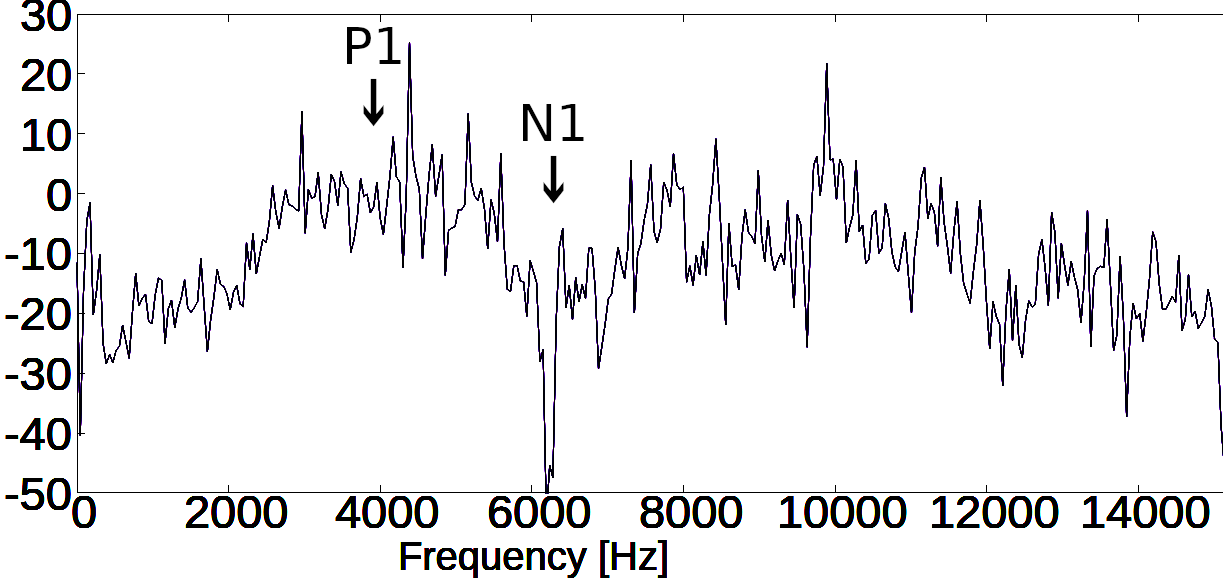
\includegraphics[keepaspectratio, scale=0.09]{picture/wn_mae_l.png}
      \subcaption{音源が前方で左耳の場合}
     
    \end{minipage} &
    \begin{minipage}[t]{0.45\hsize}
      \centering
      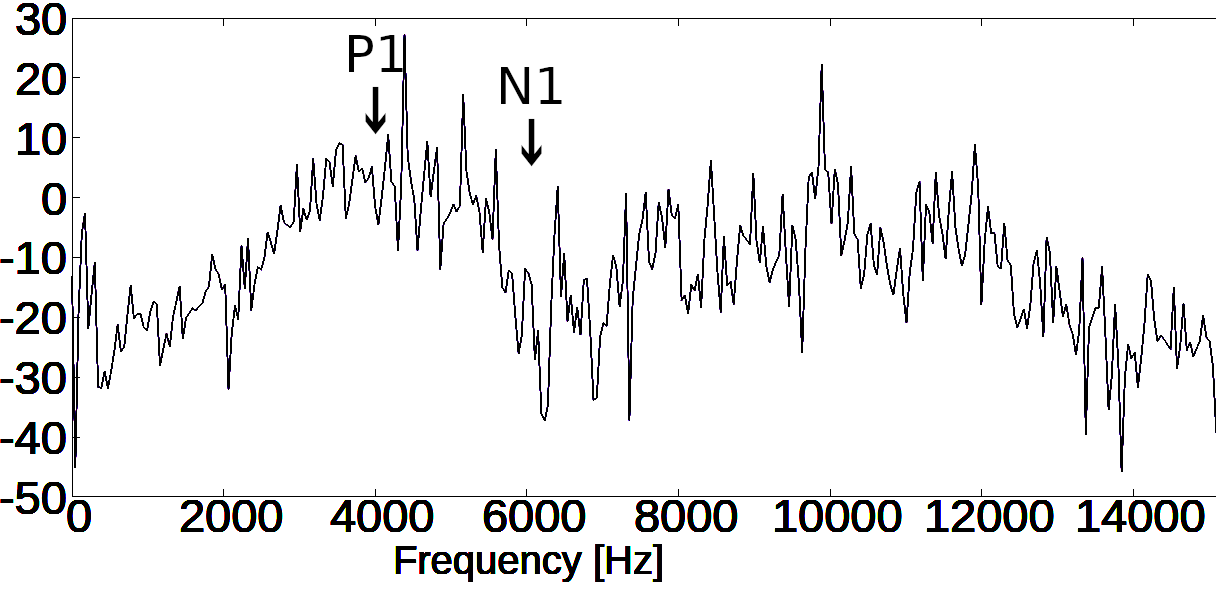
\includegraphics[keepaspectratio, scale=0.09]{picture/wn_mae_r.png}
      \subcaption{音源が前方で右耳の場合}

    \end{minipage} \\
 
    \begin{minipage}[t]{0.45\hsize}
      \centering
      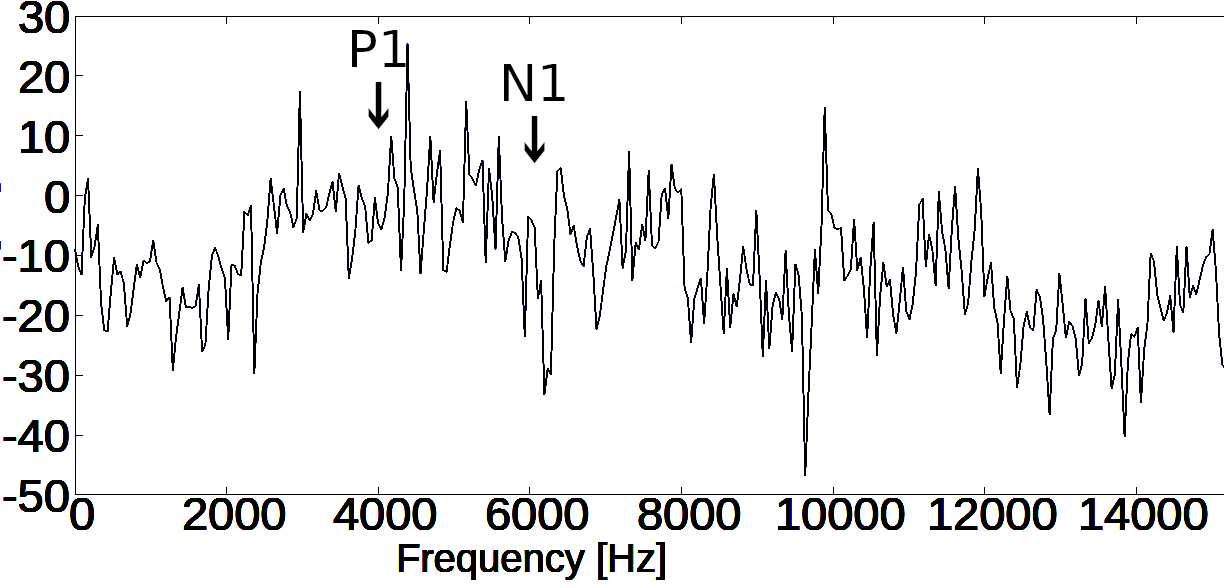
\includegraphics[keepaspectratio, scale=0.09]{picture/wn_usiro_l.png}
      \subcaption{音源が後方で左耳の場合}

    \end{minipage} &
    \begin{minipage}[t]{0.45\hsize}
      \centering
      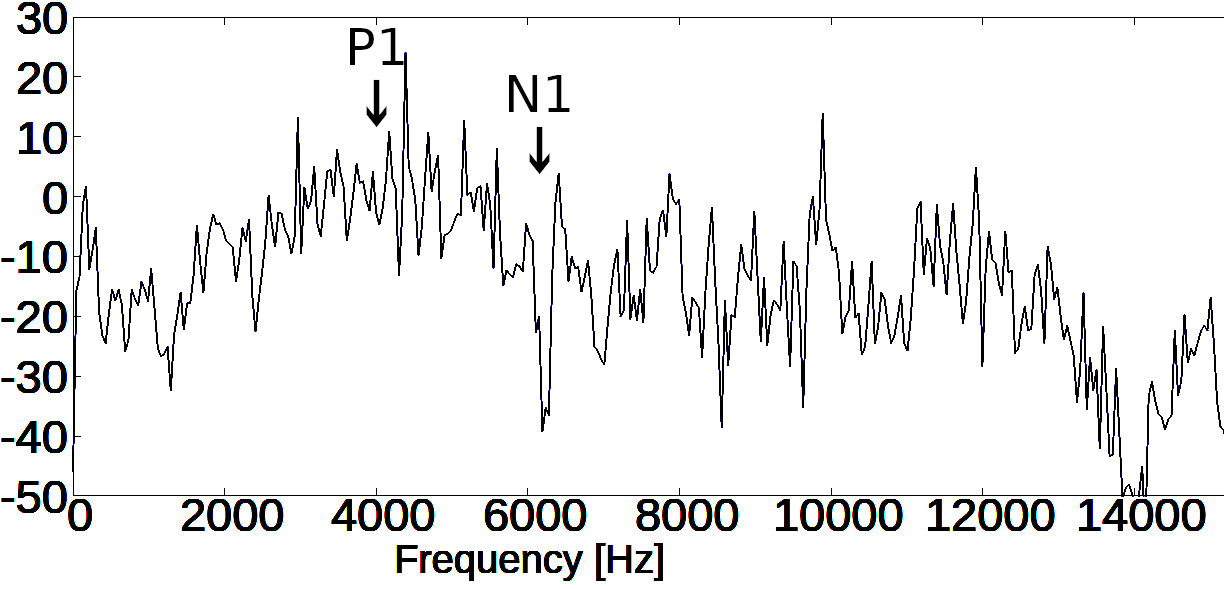
\includegraphics[keepaspectratio, scale=0.09]{picture/wn_usiro_r.png}
      \subcaption{音源が後方で右耳の場合}

    \end{minipage}
  \end{tabular}
   \caption{白色雑音を用いて測定した頭部伝達関数}\label{fig:whitenoiseHRTF}
\end{figure}

\begin{figure}[htbp]
  \begin{tabular}{cc}
    \begin{minipage}[t]{0.45\hsize}
      \centering
      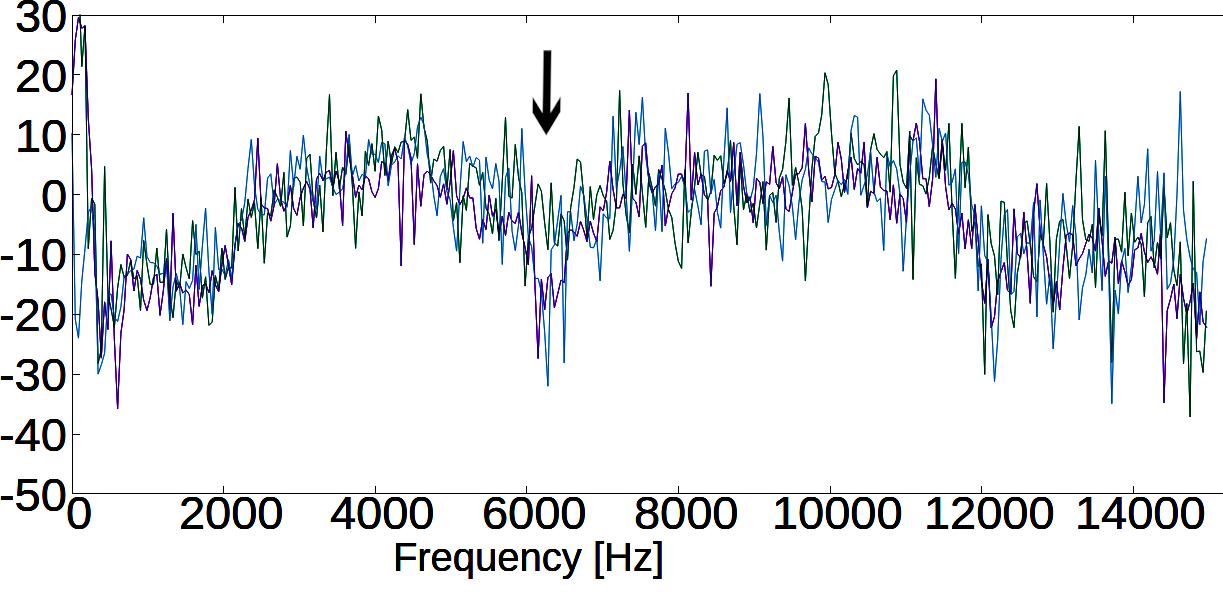
\includegraphics[keepaspectratio, scale=0.09]{picture/No1-3_mae_l.png}
      \subcaption{音源が前方で左耳の場合}

    \end{minipage} &
    \begin{minipage}[t]{0.45\hsize}
      \centering
      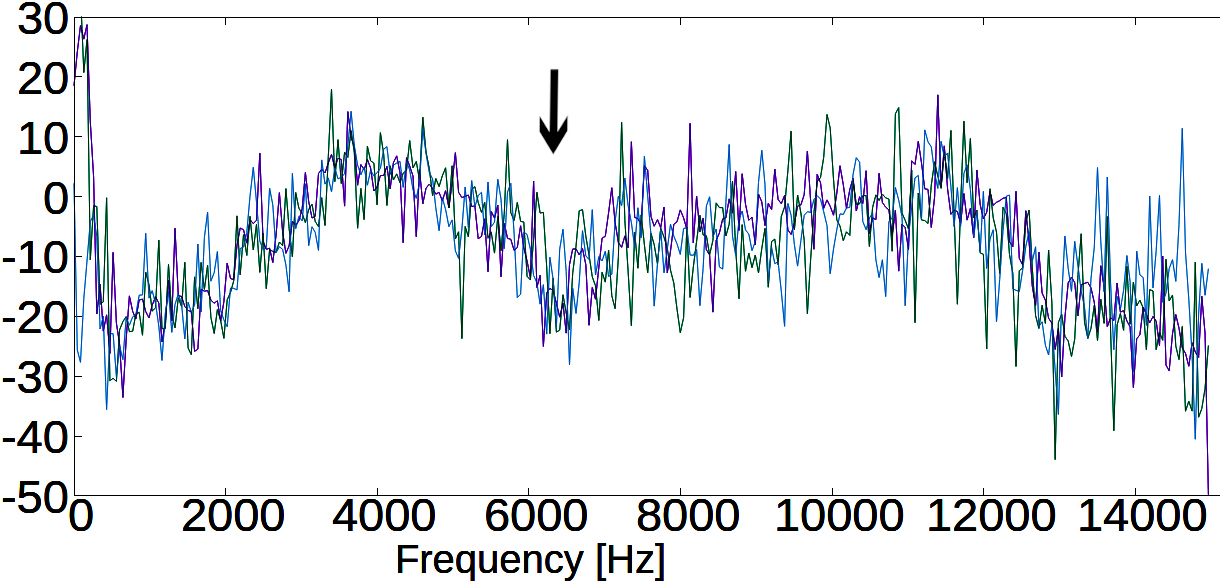
\includegraphics[keepaspectratio, scale=0.09]{picture/No1-3_mae_r.png}
      \subcaption{音源が前方で右耳の場合}
     
    \end{minipage} \\
 
    \begin{minipage}[t]{0.45\hsize}
      \centering
      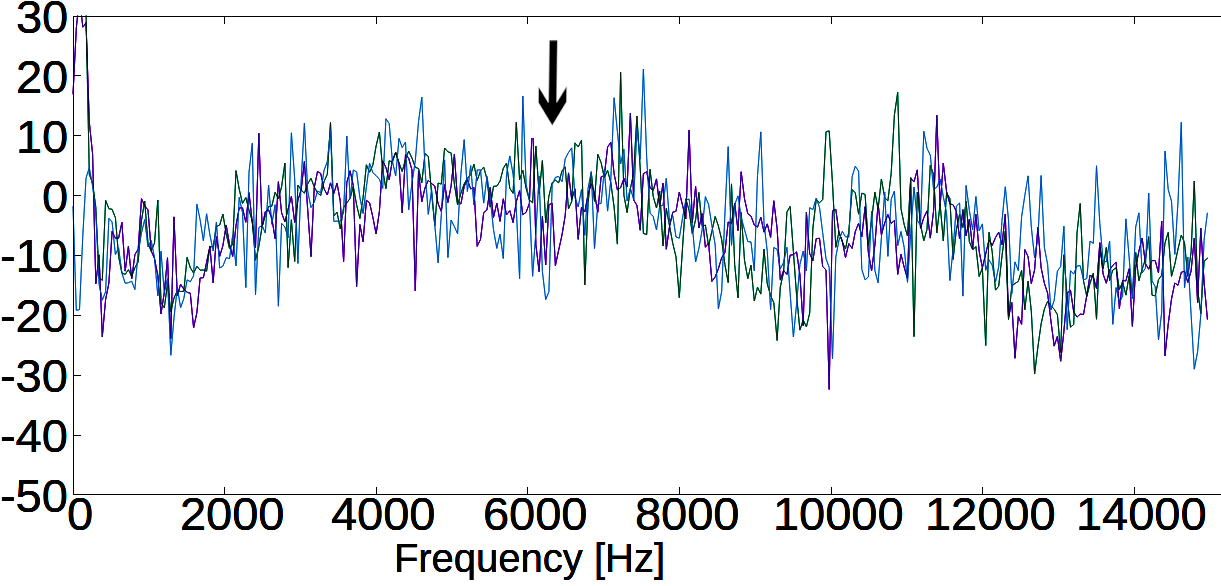
\includegraphics[keepaspectratio, scale=0.09]{picture/No1-3_usiro_l.png}
      \subcaption{音源が後方で左耳の場合}
   
    \end{minipage} &
    \begin{minipage}[t]{0.45\hsize}
      \centering
      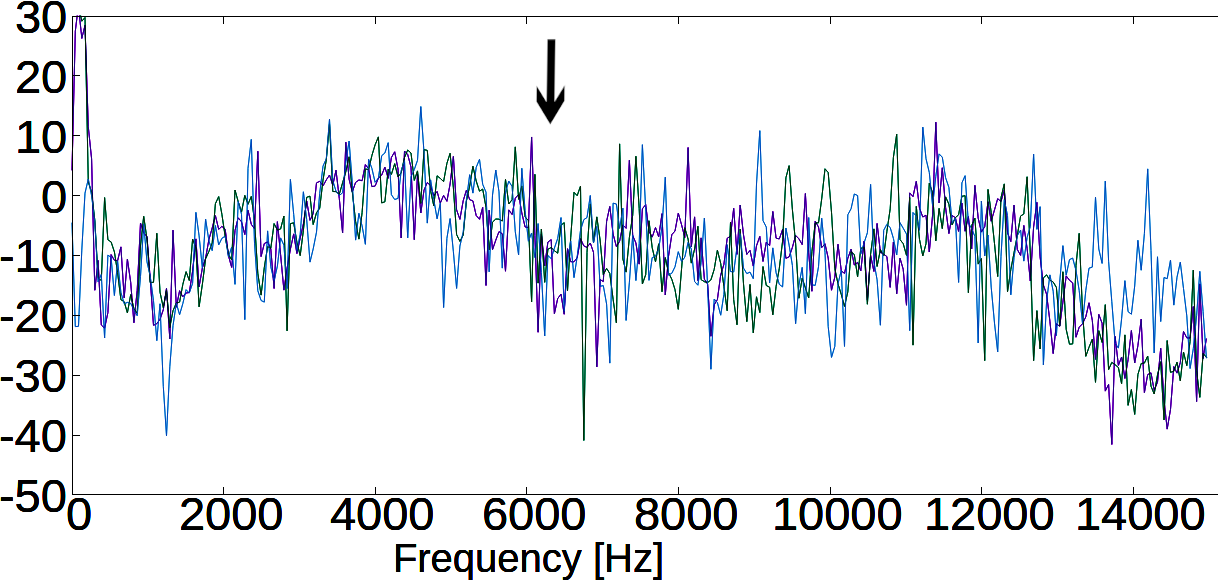
\includegraphics[keepaspectratio, scale=0.09]{picture/No1-3_usiro_r.png}
      \subcaption{音源が後方で右耳の場合}
        \end{minipage} 
  \end{tabular}
   \caption{雑用重畳録音信号から測定した頭部伝達関数}\label{fig:HRTF}
\end{figure}

%ILD
\begin{figure}[htbp]
     \begin{center}
          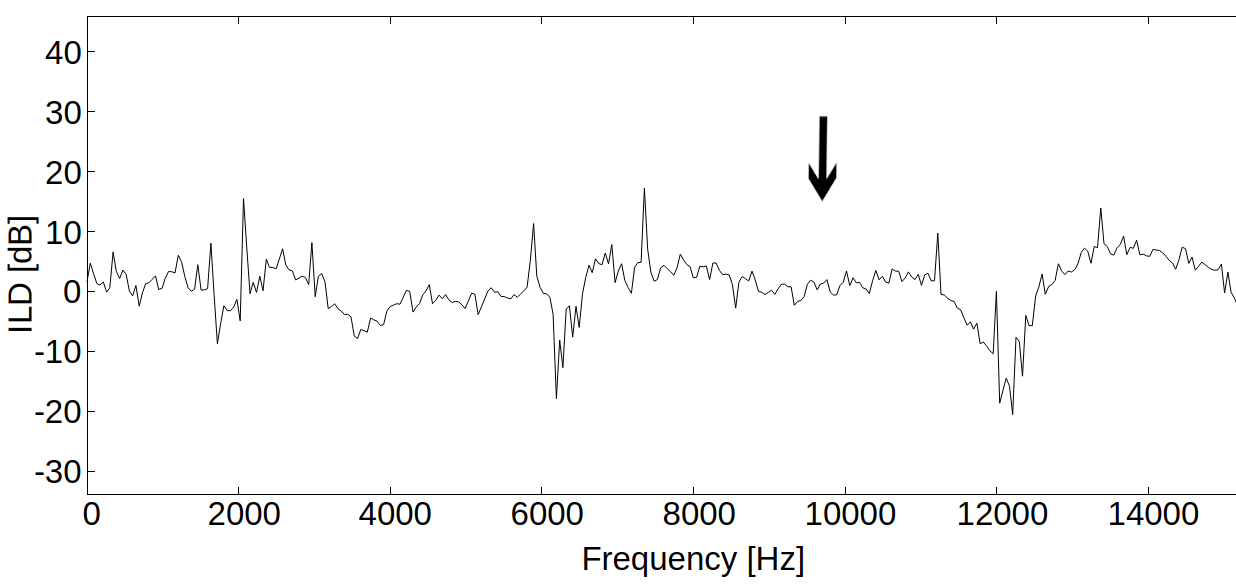
\includegraphics[clip, width=2.5in, height = 1.3in]{picture/mae_full_whitenoise.png}
          \subcaption{音源が前方の場合}
          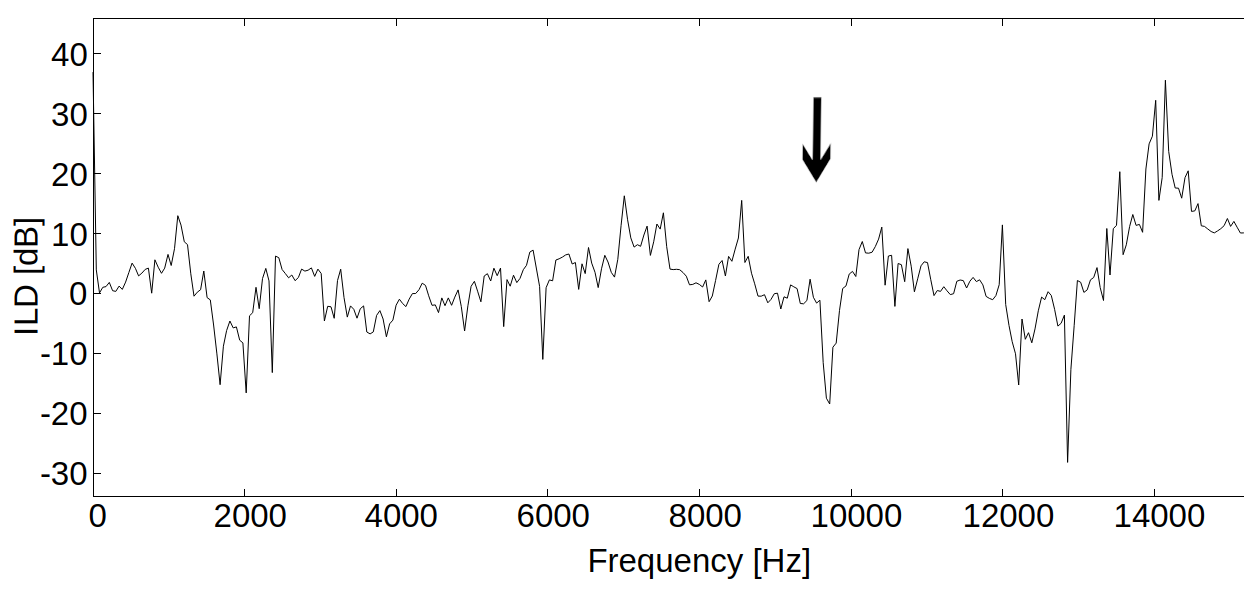
\includegraphics[clip, width=2.5in, height = 1.3in]{picture/usiro_full_whitenoise.png}
          \subcaption{音源が後方の場合}
          \end{center}
          \caption{白色雑音を用いて測定した両耳間レベル差}\label{fig:whitenoiseILD}     
\end{figure}
\begin{figure}[htbp]
    
     \begin{center}
     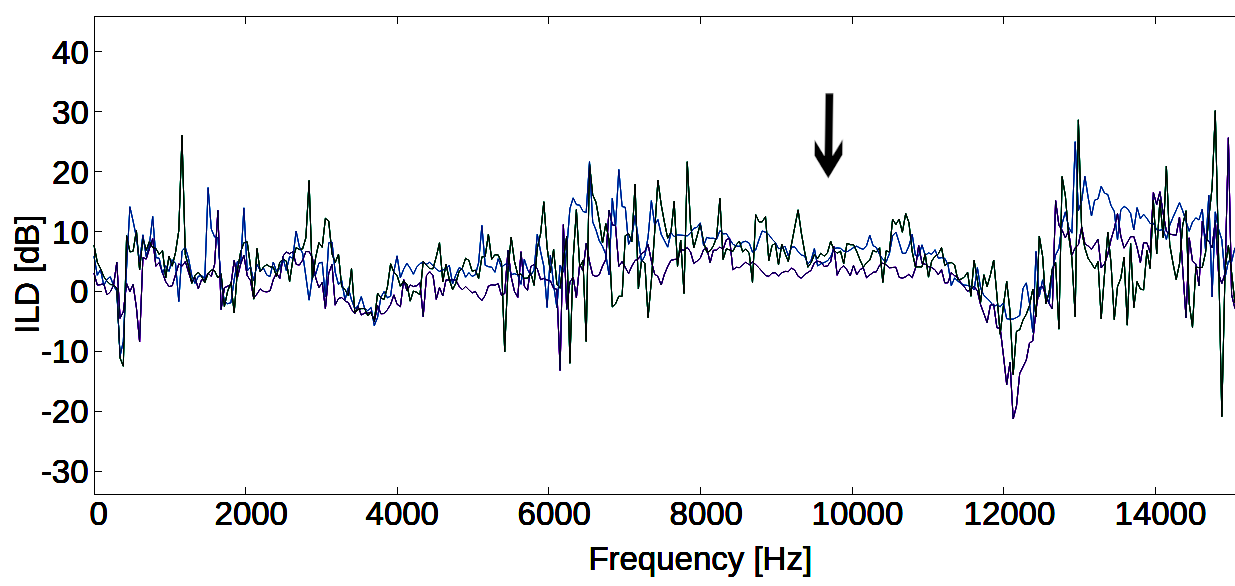
\includegraphics[clip, width=2.5in, height = 1.3in]{picture/mae_full_NoSmoothing.png}
     \subcaption{音源が前方の場合}
     
     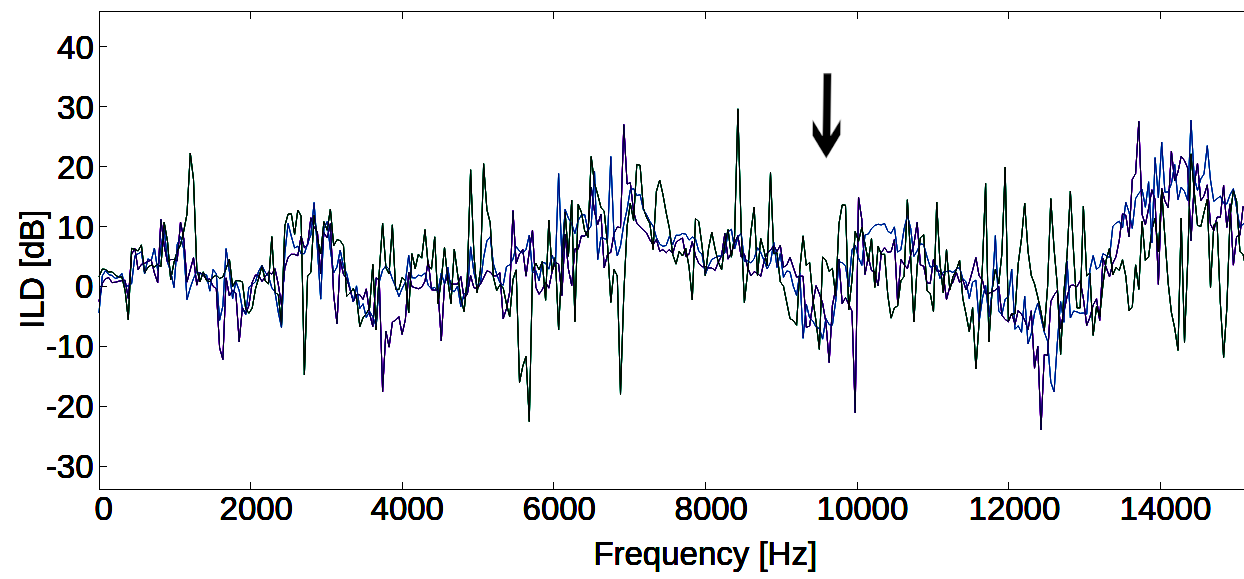
\includegraphics[clip, width=2.5in, height = 1.3in]{picture/usiro_full_NoSmoothing.png}
     \subcaption{音源が後方の場合}
     \end{center}
     \caption{雑用重畳録音信号から測定した両耳間レベル差の例}\label{fig:AILD}
\end{figure}
\end{document}
